\section{Hardware} 

\begin{figure}[ht]
    \centering
    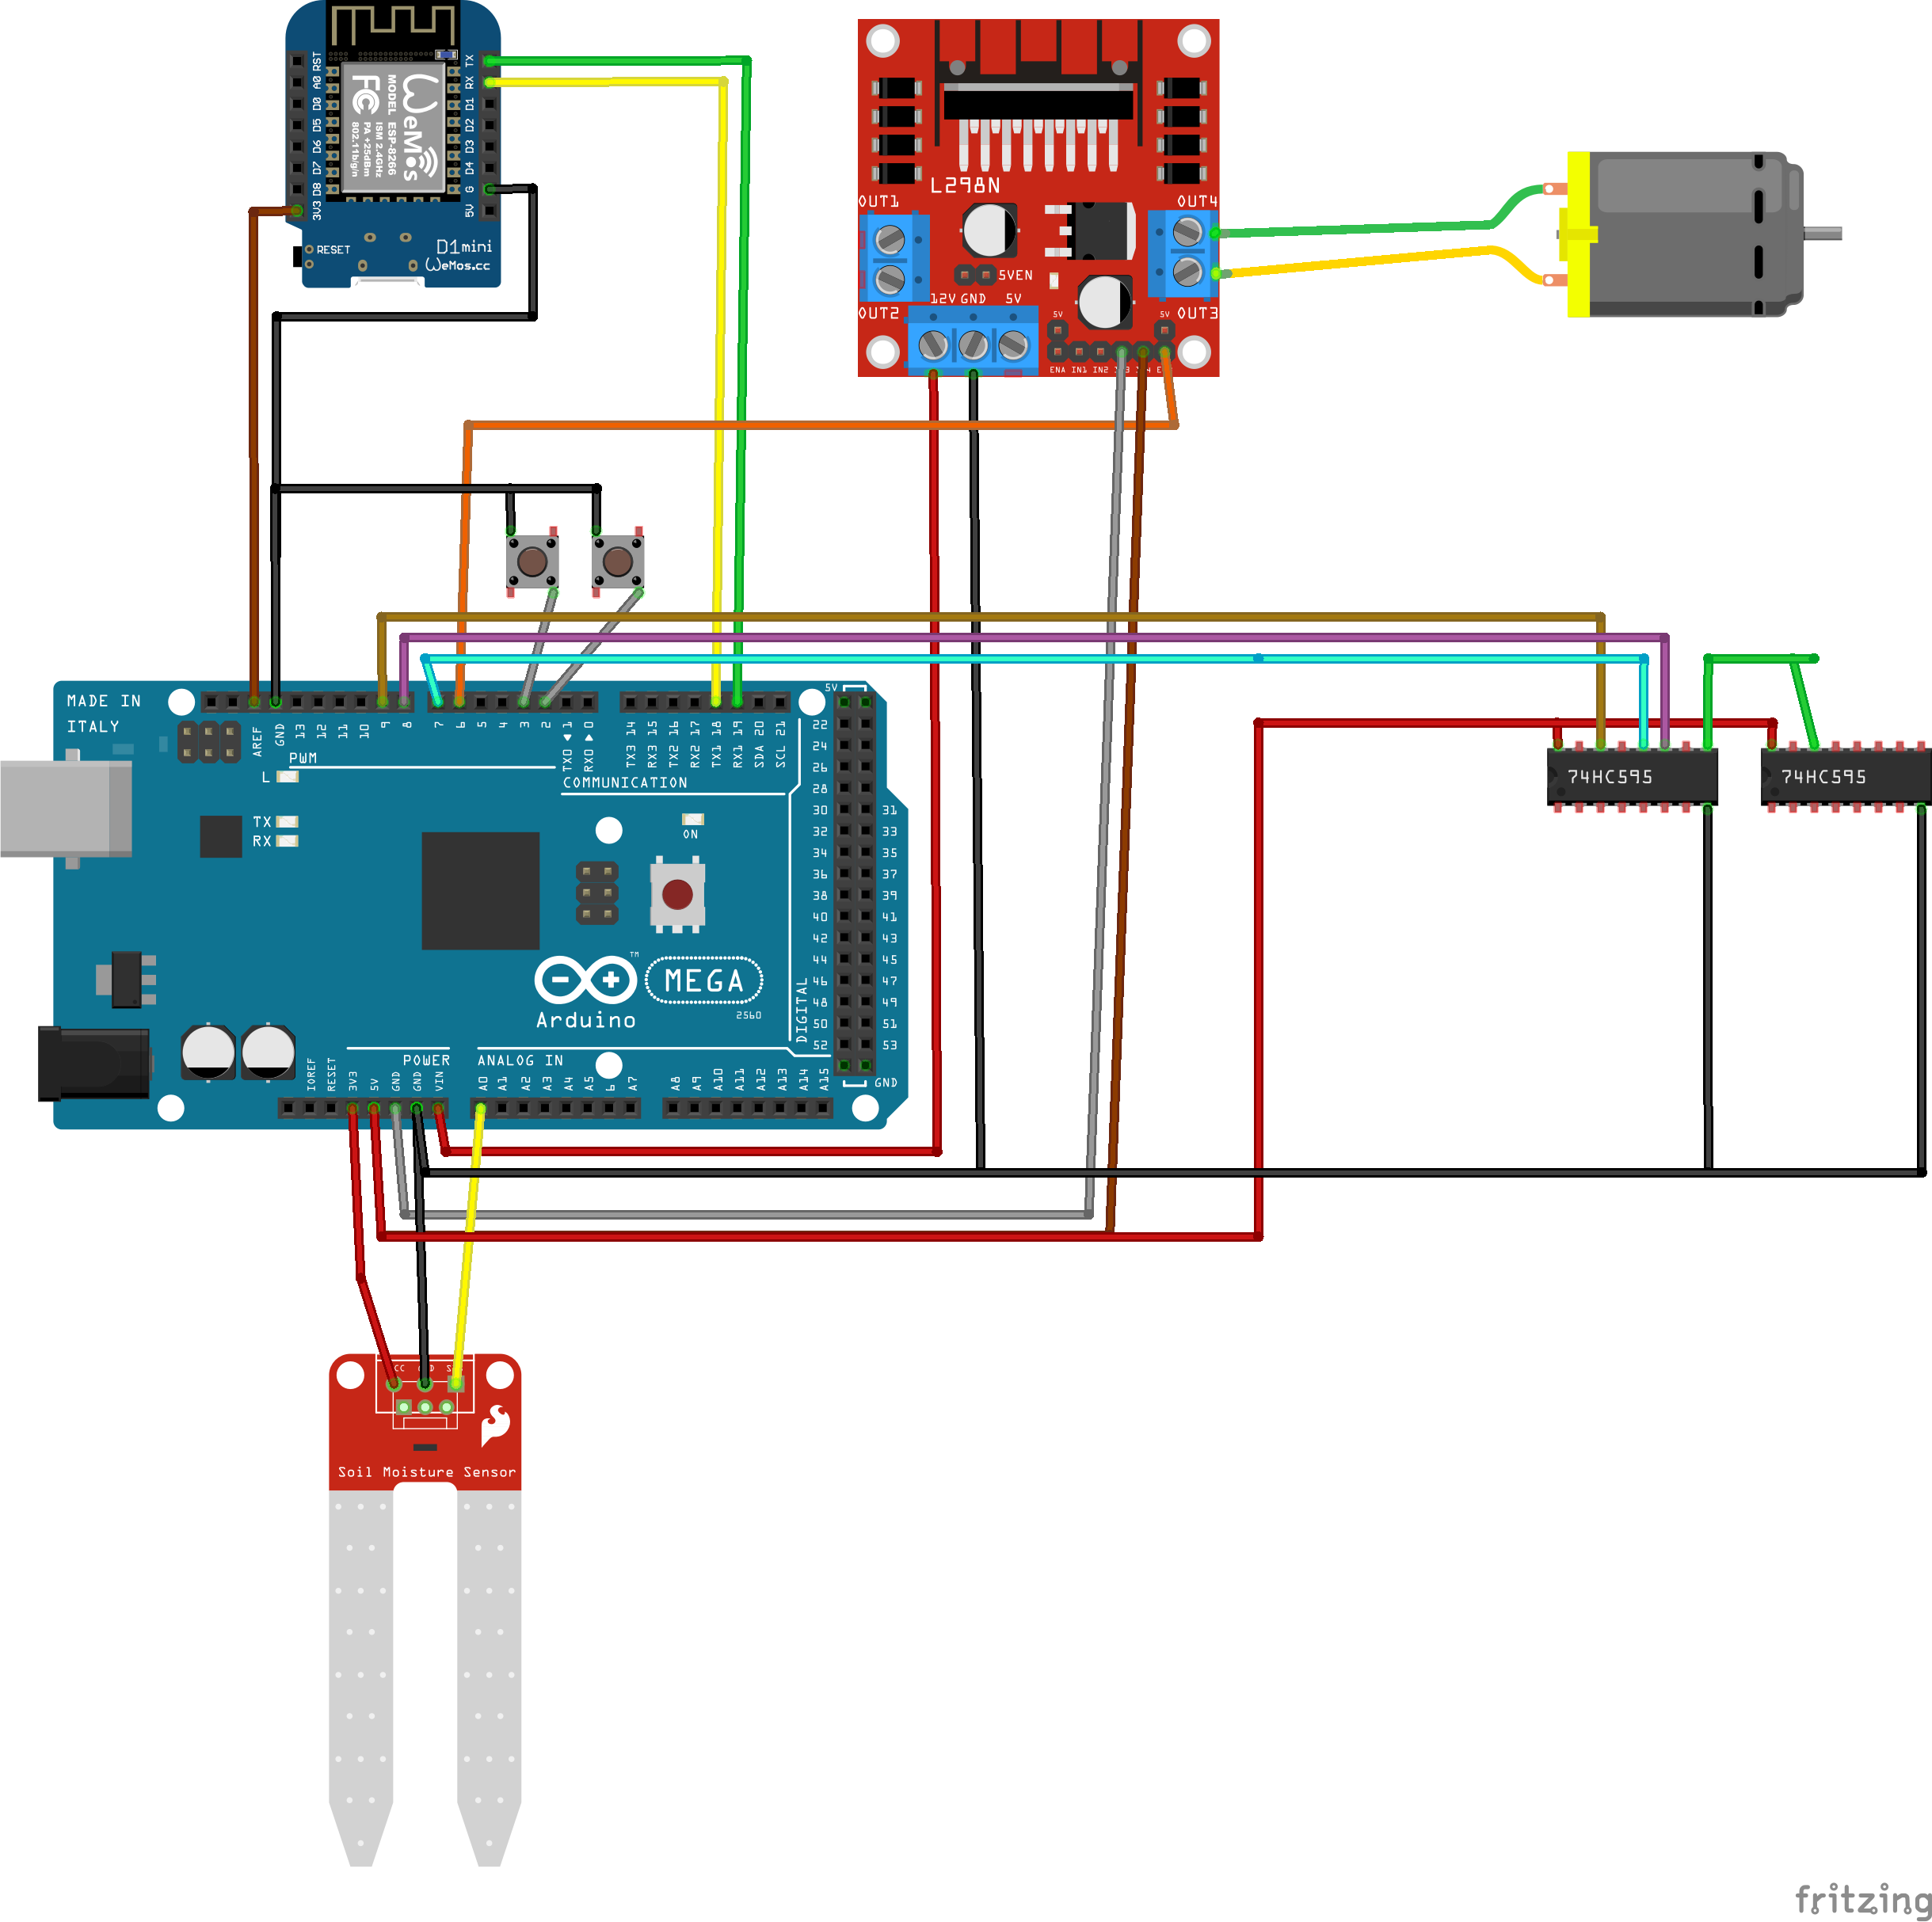
\includegraphics[width=\linewidth]{img/IrrigationStationHardware.png}
    \caption{The overview of the hardware components and their interconnections}
    \label{fig:hardware_diagram}
\end{figure}

\begin{figure}[ht]
    \centering
    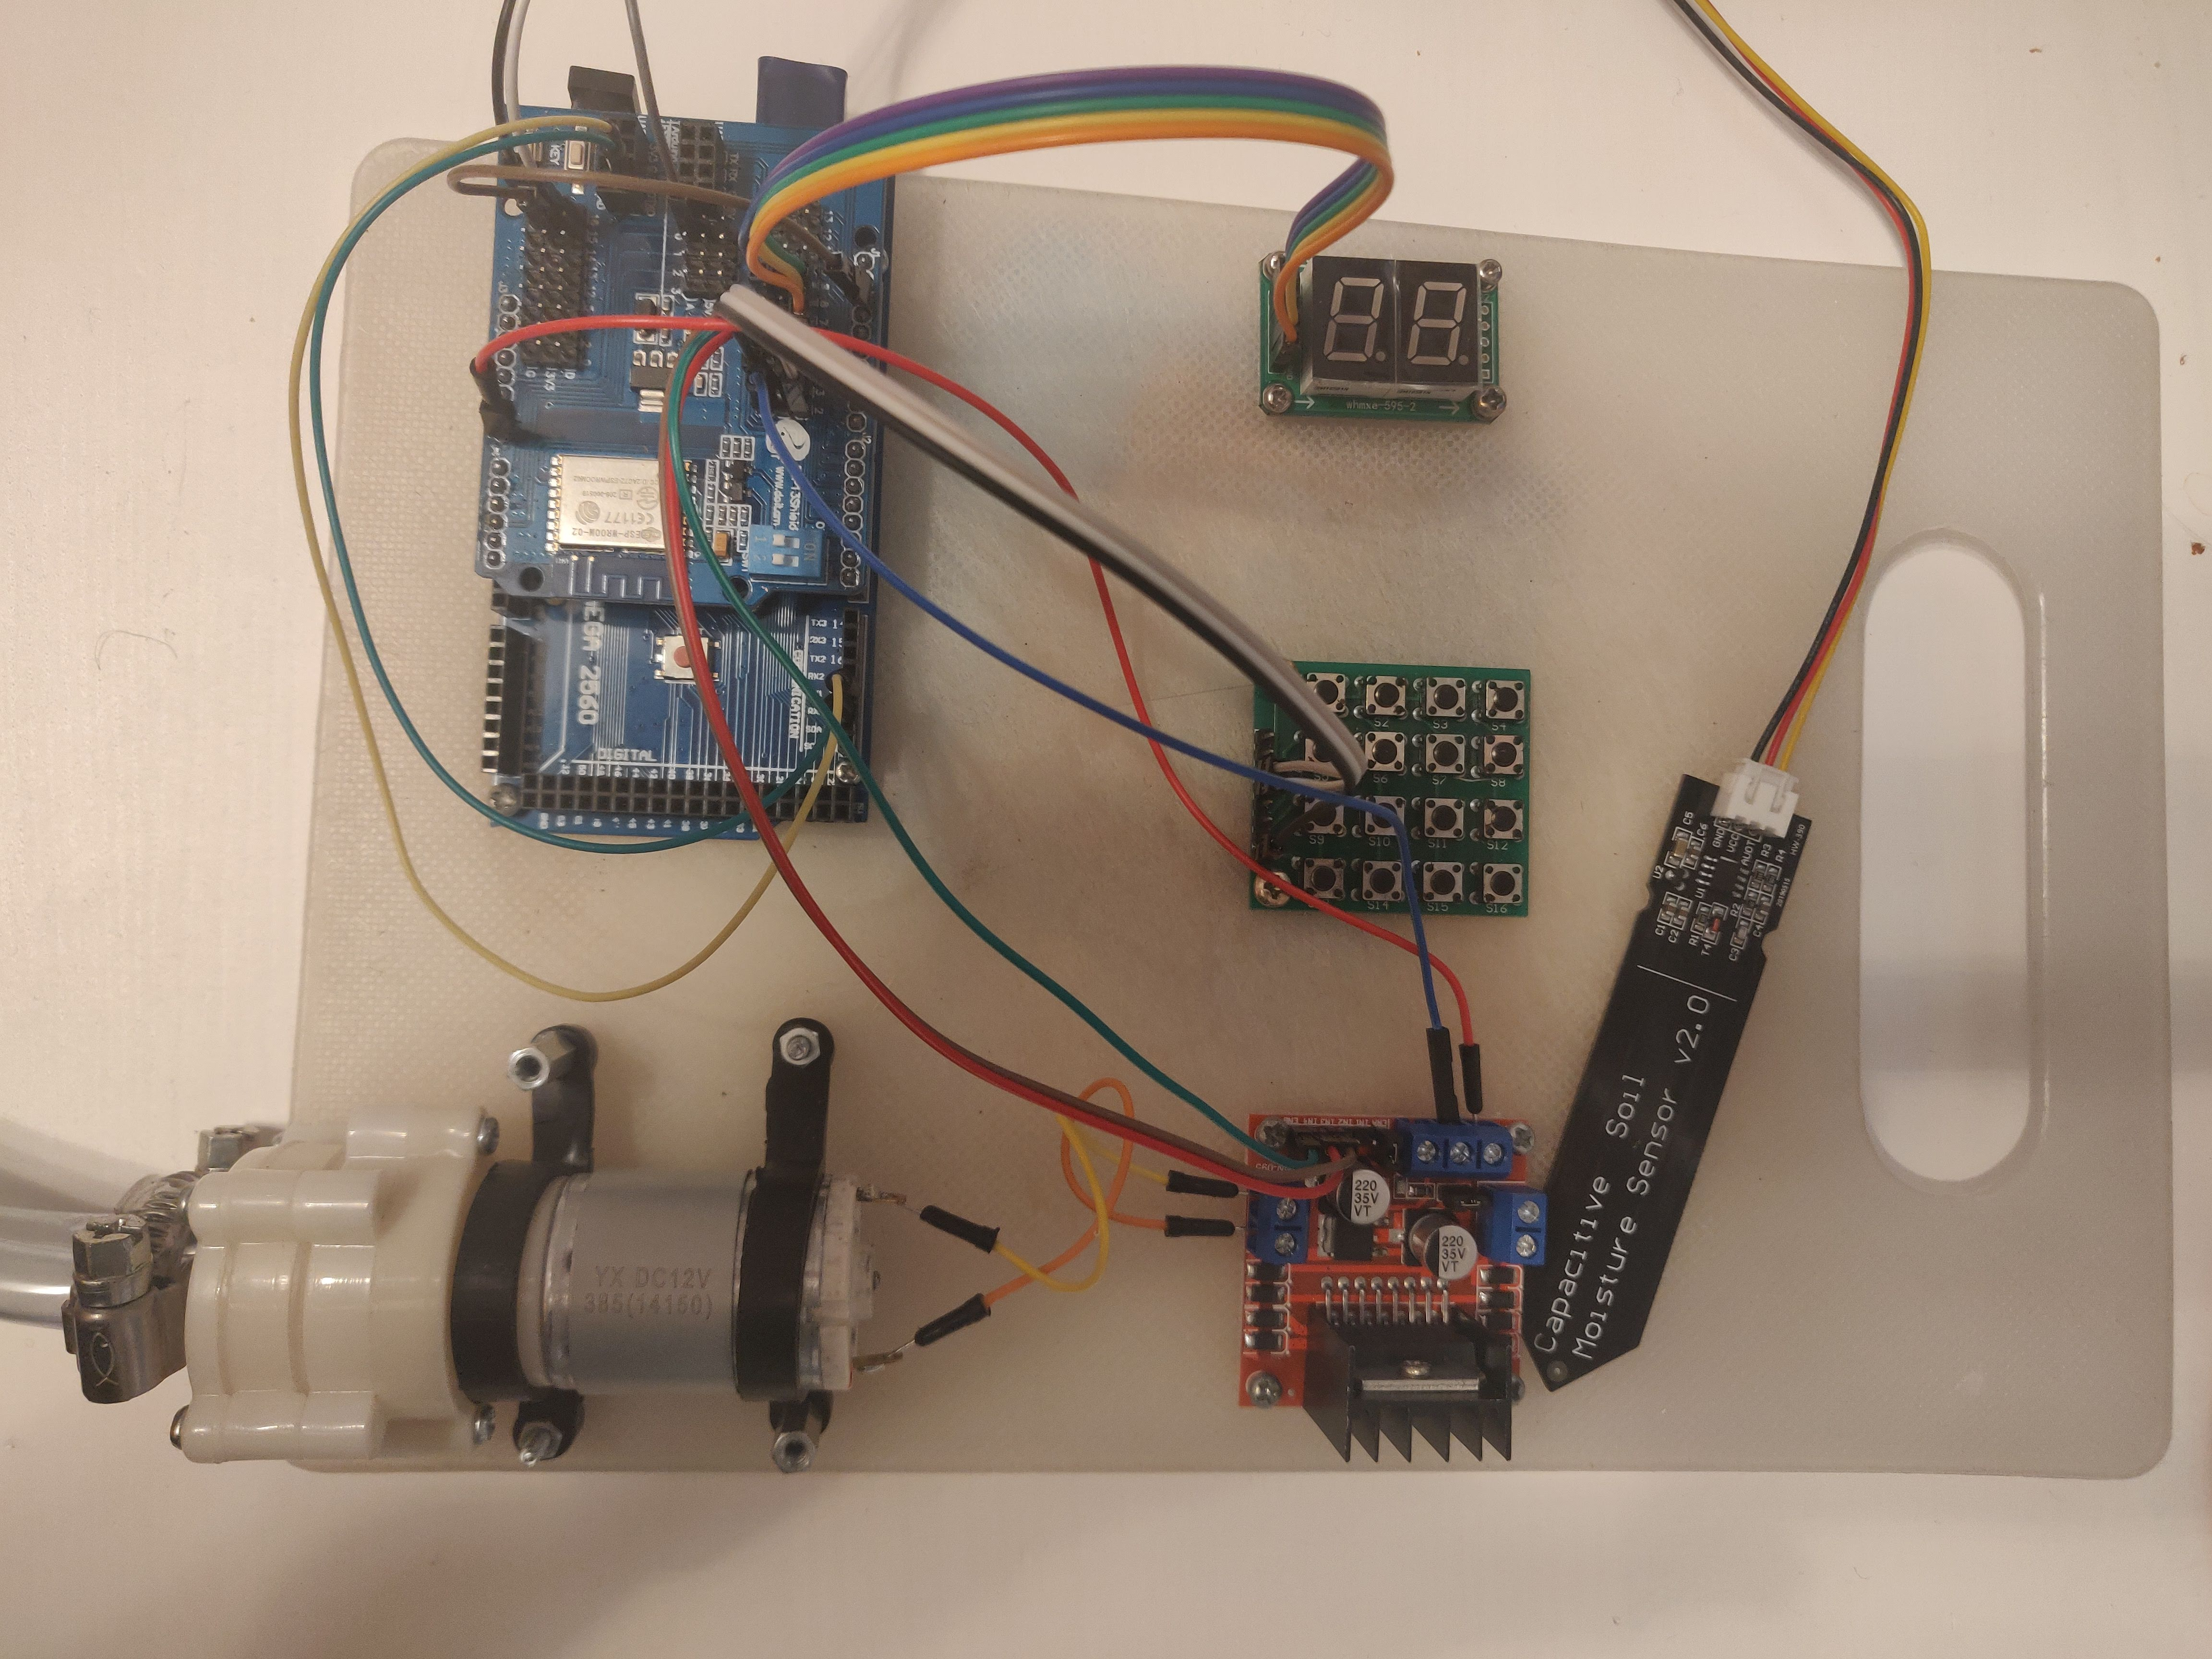
\includegraphics[width=\linewidth]{img/components.jpg}
    \caption{Picture of the components and their interconnection}
    \label{fig:components}
\end{figure}

Figure \ref{fig:hardware_diagram} shows the components used in the project. Figure \ref{fig:components} shows the real circuit.

An \textbf{Arduino Mega 2560} was used for controlling the moisture level. The program is uploaded on it. It receives 12V power through the DC jack.

For wireless communication a \textbf{DoIt ESP-13 Wi-Fi shield} was used. The AT firmware was uploaded to its ESP8266 chip. On figure \ref{fig:hardware_diagram} a different ESP component appears, because of the limitation in the design program. The voltage level shifters and regulators were hidden from the diagram because it is part of the shield. Therefore the TX and RX is directly connected to RX and TX of Arduino and the 5V port is unconnected on the image.

A 12V \textbf{water pump} was used for supplying water to the plants. This component works like a DC motor. Therefore it is represented as a motor on the image.

The pump needs a motor driver. Thus the \textbf{L298n motor driver} was added to the circuit. Its 12V power source is the external input voltage of the Arduino (VIN). The direction of the motor is hardwired, to pump only in one direction. The enable pin however is connected to the D6 pin of the Arduino board. Through this the microcontroller can turn on/off the pump or set its speed by using PWM.

A \textbf{capacitive moisture level sensor} was connected to the A0 pin of the board. It's supply voltage is 3.3V. The component differs from the one on the image because its capacitive, it is a single rod, and it can be directly connected to the board.

Two \textbf{buttons} are connected to the interrupt pins of the board. They are used for setting the extreme sensor values. When they are pressed, the program reads the sensor value and updates the current parameter with it.


Two \textbf{seven segment displays} are connected to the circuit. Their anodes are connected to '1' so the program must specify only their cathodes. The module containing the display manages this by using two 74HC595 shift registers. Therefore the only wires that are connected to the board are the: SDI, SCLK, LOAD. Thus the internal implementation of the module is not present on the diagram.
